\chapter{État de l’art}
\section{Interprétabilité et explicabilité}

\paragraph{}Dans le domaine du machine learning, les mots interprétabilité et explicabilité sont très souvent utilisés conjointement et il peut être difficile au premier abords d'en saisir la différence. De plus, il existe de nombreuses définitions différentes pour ces termes et tous les experts ne s'accordent pas forcement à ce sujet. Après l'analyse de différentes propositions, nous nous accorderons, dans ce mémoire, à donner les définitions suivantes :

\paragraph{}L'interprétabilité est le fait de pouvoir observer l'effet d'une cause dans un système c'est-à-dire de pouvoir prédire les changements dans la sortie lorsque l'on change une variable d'entrée.\par
L'explicabilité, quant à elle, est le fait d'expliquer dans des termes compréhensibles par l'homme la mécanique interne de notre système.\par
Afin de bien saisir la différence, le site \textit{KDnuggets} nous invite, dans un article\cite{kdInterpre}, à voir les choses comme si nous faisons une expérience scientifique à l'école : L'expérience peut être interprétable dans la mesure où vous pouvez voir ce que vous faites et ses effets, mais elle n'est vraiment explicable qu'une fois que vous avez creusé la chimie derrière ce que vous pouvez voir se produire.

\paragraph{}Créer un modèle interprétable implique de prendre en compte plusieurs facteurs :\par
\begin{description}
\item[Interprétabilité globale et local] L'interprétabilité d'un modèle est dite \textit{globale}, lorsque l'on comprend sa logique dans sa totalité, nous sommes donc en mesure d'en expliquer toutes les solutions. À contrario, elle sera dite \textit{local}, lorsqu'il est possible d'expliquer seulement une ou plusieurs solutions spécifiques. Un problème complexe pourra ainsi être découpé en un sous problème plus simple afin de pouvoir expliquer une partie des solutions comme le montre la figure \ref{globalVSlocal} ci-dessous. Sur cette figure, nous voyons à gauche la totalité du problème où les parties en bleu et en rouge correspondent aux domaines de prédiction de deux classes et où les croix et les ronds correspondent à des instances spécifiques de notre problème. On voit donc que le problème n'est pas linéaire et est assez complexe. Fournir une explication global à notre modèle de prédiction serait donc compliqué et pas forcement pertinent, or nous pouvons voir que la majorité des instances spécifiques se trouvent sur un problème simple et linéaire. L'explication local consiste donc à fournir une explication uniquement aux instances correspondantes à notre problème linéaire.
\begin{figure}[h]
\centering
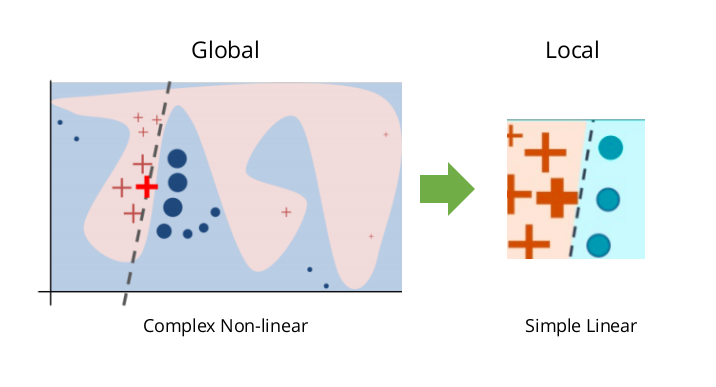
\includegraphics[scale=0.4]{src_img/globalVSlocal.png}
\caption{Un problème global complexe pouvant être expliqué à échelle local. \textit{Source : \cite{limePaper}}}
\label{globalVSlocal}
\end{figure}

\item[Limatation temporel] Le temps que l'on peut allouer pour fournir une explication à notre modèle est aussi à prendre en compte. En effet, fournir une explication peut prendre du temps et cette explication peut être longue à appréhender pour un être humain. Dans certains contextes où la prise de décision devra être effectuée rapidement, il sera préférable d'avoir une explication simple, compréhensible et fournis rapidement par la machine. Dans d'autres cas, nous pourrons prendre le temps d'aborder une explication plus complexe et détaillée.

\item[La cible de l'explication] La nature de l'expertise de l'utilisateur est aussi un facteur à prendre en compte dans le choix de l'explication que nous voulons lui apporter. En effets, un expert dans le domaine aura tendance à préférer une explication exhaustive et précises qu'une explication simple et opaque et inversement pour une personne moins à l'aise.
\end{description}

\textbf{Pré-requis d'un modèle interprétable :}\\

En plus de prendre en compte les facteurs précédemment évoqués, un modèle interprétable doit être capable de satisfaire une liste de choses souhaitées. L'article "A survey of methods for explaining black box models"\cite{surveyExplaining} met en avant, après une analyse de différents états de l'art traitant de ce sujet, les desiderata d'un modèle interpretable :
\begin{description}
\item[Interpretabilité] Dans quelle mesure le modèle ou la prédiction sont compréhensifs par l'homme. Ce sujet est encore en débat afin de savoir comment mesurer cette interprétabilité.

\item[Précision] Dans quelle mesure le modèle interprétable prédit avec précision les différentes instances. La précision d'un modèle peut être faite avec le \textit{score de précision} (accuracy score), il s'agit simplement d'un rapport entre les observations correctement prédites et les observations totales. La précision est l'indicateur de base afin de calculer la précision d'un modèle, ce score fonctionne mieux si les faux positifs et les faux négatifs ont un coût similaire. Si le coût des faux positifs et des faux négatifs est très différent, il vaut mieux regarder le \textit{F1-score}. Le F1-score est la moyenne pondérée de la précision et du rappel.
\[
F1 Score = 2*\frac{Recall * Precision}{Recall + Precision}
\]
Où la \textit{précision} est le rapport des observations positives correctement prédites au total des observations positives prévues. Et le \textit{recall} (rappel) est le rapport des observations positives correctement prédites à toutes les observations dans la classe réelle.

\item[Éthique] Si notre modèle traite des données personnelles, il devra garantir en plus une protection contre toutes formes de discrimination ainsi qu'une protection de la vie privée des personnes concernées.\\
\end{description}

\paragraph{}Ces différents aspects jouent un rôle important quant à la confiance qu'un utilisateur va apporter à notre modèle interprétable. De plus d'autres notions viennent s'ajouter, notamment pour les modèles d'exploration de données et d'apprentissage automatique. Il est important de respecter des critères tels que la \textit{robustesse}, la \textit{causalité}, l'\textit{évolutivité} et la \textit{généralité}. Cela signifie qu'un modèle doit garantir un certain niveau de performance indépendamment des données d'entrée (robustesse), et que les changements d'entrée dû à une perturbation affectent le comportement du modèle (causalité). Enfin, étant donné que nous pouvons utiliser le même modèle avec une multitude données d'entrée et dans différents cas d'applications, il est préférable d'avoir des modèles portables possédant un minimum de restriction (évolutivité, généralité).

\section{Ouvrir les boites noires}
\paragraph{}Cette section se base principalement sur l'article "A survey of methods for explaining black box models"\cite{surveyExplaining} qui passe en revue cinquante-quatre méthodes aillant pour but d'ouvrir différentes boites noires, en nous fournissant une classification exposée dans un tableau disponible en annexe 1 et 2. Cette revue permet de distinguer différents types de problèmes, d'explicateurs, de boites noires, de données d'entrée ainsi que différentes restrictions sur le modèle. Mais cette section est aussi complétée autre autre par le livre de Christoph Molnar "Interpretable Machine Learning" \cite{molnar2019} résumant l'essence de l'interprétabilité dans le machine learning et différentes autres ressources citées dans cette section. Nous allons commencer par expliquer les différentes caractéristiques.

\subsection{Types de problèmes}
\paragraph{}Nous pouvons distinguer deux grand types de problèmes. Le premier, la rétro-ingénierie, consiste à trouver une explication à un modèle déjà existant. Pour cela, nous allons utiliser des algorithmes externe à notre modèle afin de déduire une explication. Ce type de problème sera divisé en trois sous-problèmes : explication du modèle, explication du résultat et inspection de la boîte noire. Le second type de problème consiste à créer directement un modèle prédictif interprétable qui nous fournira une explication à ses résultats de lui même.
\subsubsection{Explication du modèle}
\paragraph{}Ce problème consiste à fournir un modèle interprétable et transparent capable d'imiter le comportement d'une boite noire et de nous fournir un prédicat compréhensible par l'homme.\\
Étant donnée un prédicateur de boite noire b et un ensemble de données D, le problème d'explication du modèle consiste à trouver une fonction f telle que f(b,D)=c où c est un prédicateur compréhensible capable d'imiter le comportement de b et dérivable afin d'obtenir une explication.

\subsubsection{Explication du résultat}
\paragraph{}Ce problème consiste à fournir un résultat interprétable, c'est-à-dire que le modèle devra fournir le résultat avec une explication sur les raisons qui l'ont poussé à donner cette prédiction. Il n'est pas nécessaire d'expliquer la logique interne du système mais seulement le processus de décision pour une instance donnée (interprétation local).

\subsubsection{Inspection de la boîte noire}
\paragraph{}Ce problème consiste à fournir une représentation visuelle ou textuelle afin de comprendre le fonctionnement interne de notre boite noire (interprétation globale).\\
Étant donnée un prédicateur de boite noire b et un ensemble de données D, le problème d'explication du modèle consiste à trouver une fonction f telle que f(b,D)=V où V est une représentation du fonctionnement de la boite noire.

\subsubsection{Conception transparente}
\paragraph{}Ce problème consiste à créer un modèle prédictif transparent qui soit directement interprétable globalement ou localement. Il fournira donc de lui même une explication à ses prédictions sans que l'ont ai besoin d'utiliser des algorithmes externe à notre modèle.

\subsection{Types d'explicateurs}
\paragraph{}Il existe différentes méthodes afin de fournir une explication à un modèle type boîte noire, nous allons dans cette sous-section présenter les principales :
\begin{itemize}
    \item \textbf{Arbre de décision (Decision Tree)} : L'arbre de décision exploite un arbre qui a pour noeuds des conditions, les arcs correspondent à la valeur d'une variable d'entrée et les feuilles correspondent aux différents labels possible. La figure \ref{decision_tree} montre un exemple trivial d'arbre de décision. Ainsi, la décision sera simplement expliquée en exprimant les chemins de l'arbre empruntés. 

    \begin{figure}[h]
    \centering
    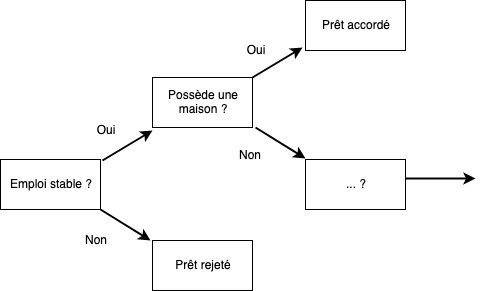
\includegraphics[scale=0.5]{src_img/decision_tree.jpg}
    \caption{Exemple d'un arbre de décision}
    \label{decision_tree}
    \end{figure}
    
    \item \textbf{Règles de décision (Decion Rules)} : Utilisé pour expliquer le modèle, le résultat ainsi que pour la conception transparente. Il est aussi possible de transformer un arbre en un ensemble de règles. Les règles de décisions sont simplement des conditions IF-THEN : 
    
    if condition1, condition2, condition3 then outcome 
    
    \item \textbf{Importance des variables (Features Importance)} : Solution souvent utilisée, elle consiste à trouver les entrées de la boite noire pour lesquelles les poids sont les plus importants. Par exemple, pour une classification d'image, de trouver les pixels dans l'image jouant un rôle important dans notre prédiction prédiction. Comme le montre la figure \ref{chickenPixel} tirée de l'article \textit{"Explainable Artificial Intelligence: Understanding, Visualizing and Interpreting Deep Learning Models"} \cite{explainingIA}.\\
    \begin{figure}[h]
        \centering
        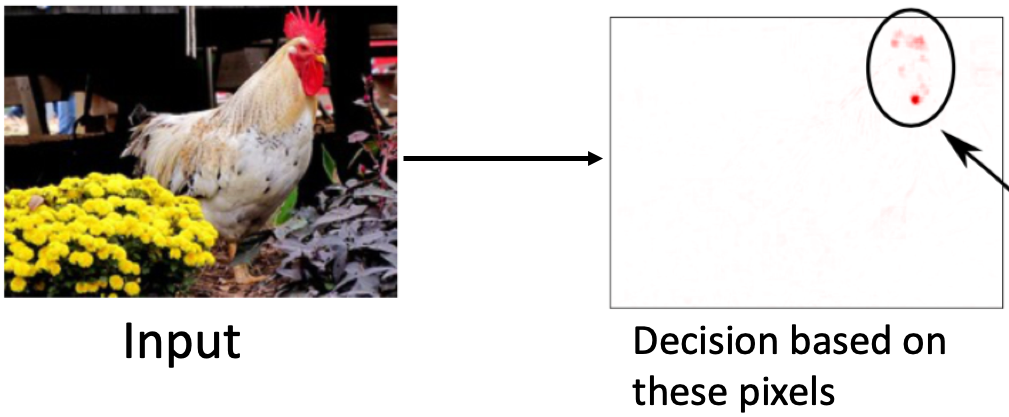
\includegraphics[scale=0.35]{src_img/chickenPixel.png}
        \caption{Importance des fonctionnalités : explication de la prédiction "coq"}
        \label{chickenPixel}
    \end{figure}
    
    \item \textbf{Salient Mask} Généralement utilisé pour expliquer localement les réseaux de neurones profond (DNN), le salient mask permet de mettre en évidence visuellement les parties déterminantes de l'entrée analysée. L'article \textit{"Real Time Image Saliency for Black Box Classifiers"}\cite{silentMask} décrit son fonctionnement et la figure \ref{silentMaskExemple} montrant un exemple de salient mask est tirée de cet article.
    \begin{figure}[h]
        \centering
        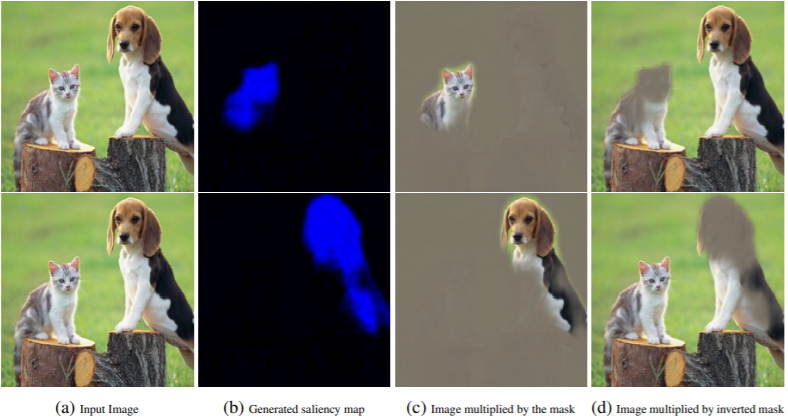
\includegraphics[scale=0.85]{src_img/silentMaskExemple.PNG}
        \caption{Masque saillant : explication de la prédiction chien et chat}
        \label{silentMaskExemple}
    \end{figure}
    
    \item \textbf{Analyse de sensibilité (Sensitivity Analysis)} : Généralement utilisée pour l'inspection de boite noire. L'analyse de sensibilité consiste à évaluer l’incertitude statistique du résultat d’une boîte noire avec les différentes sources d’incertitude dans ses entrés. En d'autres termes, cela consiste à modifier des variables d'entrées afin de voir si cela a un impact sur le résultat en sorti et donc de savoir comment elles affectent notre prédiction.
    
    \item \textbf{Diagramme de dépendance partielle (Partial Dependence Plot)} : Ces graphiques permettent de comprendre l'effet d'une ou deux variables d'entrée sur la sortie du modèle. Le but étant de  montrer si la relation entre une caractéristique d'entrée et la sortie est linéaire, monotone ou plus complexe. Par exemple, appliqué à un modèle de régression linéaire, les tracés de dépendance partielle montrent toujours une relation linéaire. Nous somme limité par une ou deux variables à la fois, car une variable donne une représentation en 2 dimensions du problème et deux variables fournissent donc une représentation 3 en dimensions. Par exemple, la figure \ref{partialDependencePlot} tirée du livre \cite{molnar2019} montre trois diagrammes de dépendances différents sur trois valeurs d'entrées (la température, l'humidité et la vitesse du vent) et leurs impactes linéaire sur la prédiction du nombre de vélos.
    \begin{figure}[h]
        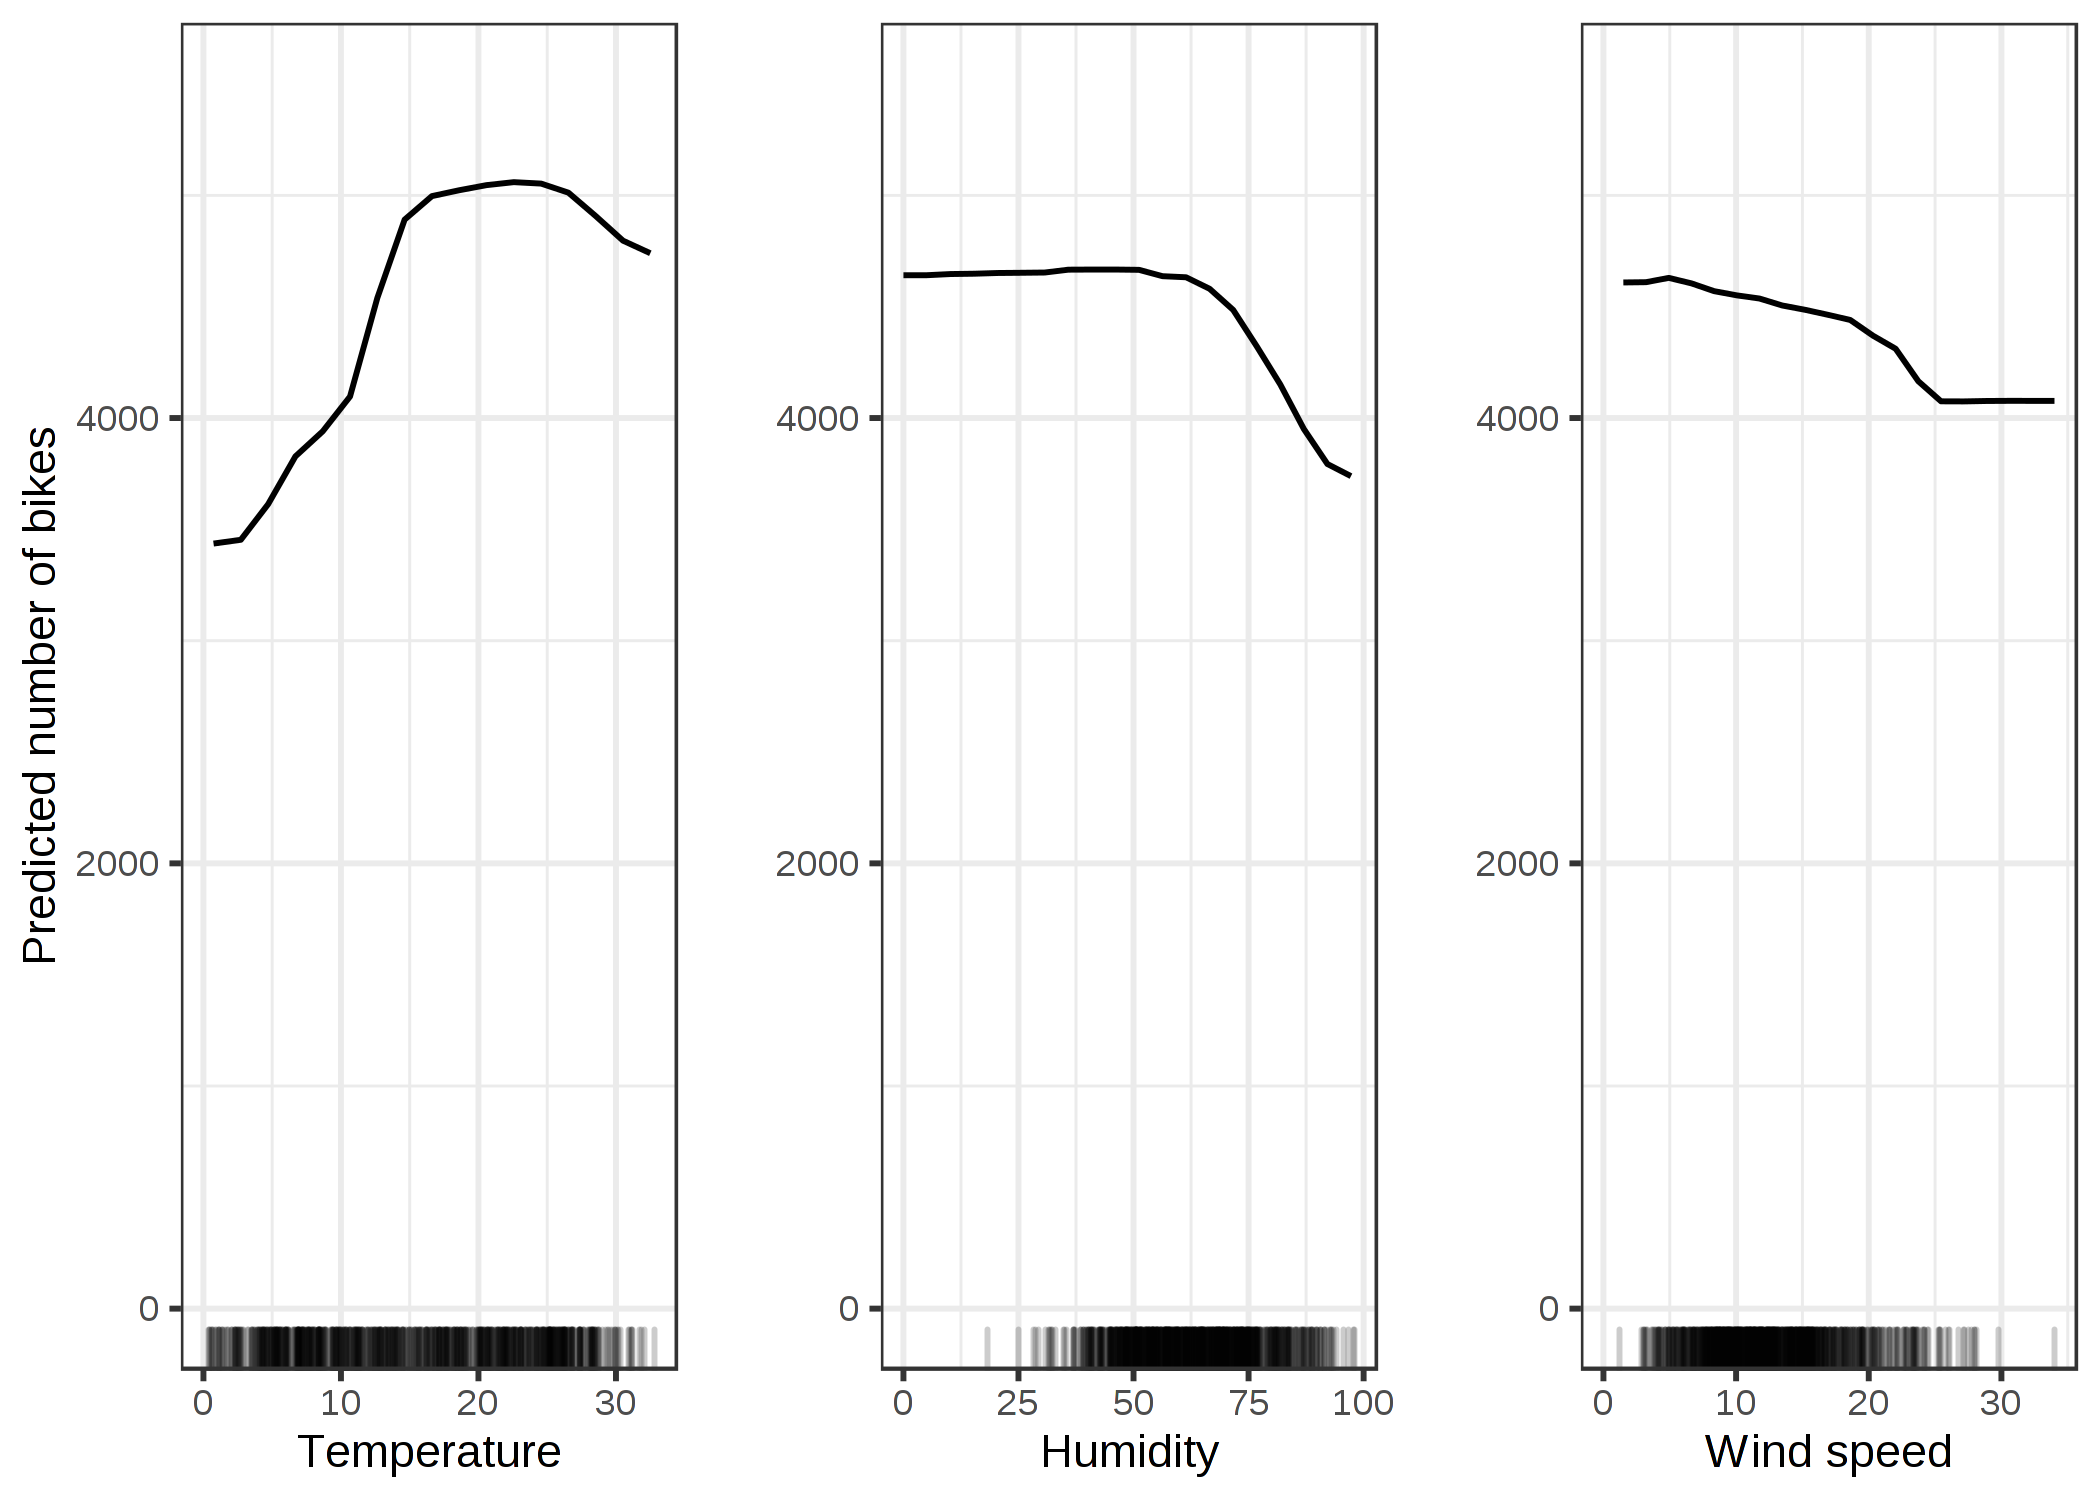
\includegraphics[scale=0.17]{src_img/partialDependencePlot.png}
        \caption{Exemple de diagramme de dépendance partielle.}
        \label{partialDependencePlot}
    \end{figure}
    
    \item \textbf{Sélection de prototype (Prototype Selection)} : Cet explicateur consiste à retourner, avec le résultat, un exemple très similaire à l'enregistrement classifié, afin de préciser avec quel critère la prédiction a été renvoyée.
    
    \item \textbf{Activation des neurones (Neurons Activation)} : L'analyse d'un réseau de neurones permet aussi de comprendre son comportement. Cela consiste à analyser les neurones activés ou non pour chaque entrés passées en argument à notre modèle.
\end{itemize}

\subsection{Spécificité de la boite noire}
\paragraph{}Le type d'explicateur à utiliser dépend aussi de notre boite noire, de ses restrictions et des données d'entrée utilisées. Nous distinguons principalement trois types de données d'entrées : les données tabulaires, textuelles et les images.

\subsubsection{Données d'entrées}
\begin{itemize}
    \item \textbf{Tabulaire :} Dans une donnée tabulaire, chaque enregistrement partagent le même ensemble de caractéristiques qui sont de type textuel, numérique ou booléen. La donnée la plus couramment utilisée est le fichier csv.
    
    \item \textbf{Image :} Le modèle prévisionnel le plus couramment utilisé est la prédiction d'image, cela comprend aussi l'exploitation de vidéos. Pour pouvoir être traité, l'image est transformée en une liste nombres de la taille de l'image (hauteur x largeur) où chaque nombre de la liste correspond à la couleur d'un pixel. Ces images peuvent être traitées telles quelles par la boite noire ou être pré-traitées afin qu'elles aient toutes la même taille ou de leur appliquer un filtre par exemple.
    
    \item \textbf{Textuel :} Souvent utilisé pour le traitement automatique du langage naturel (NLP), cette donnée est logiquement dépendante de la langue utilisée à l'entrainement de notre boite noire (un modèle entraîné en français ne pourra pas prendre un texte anglais en entrée). Un exemple serai un modèle de classification de sujet ou bien de détection de spam dans une boite mail.
\end{itemize}

\subsubsection{Type de boites noires}
\paragraph{}Dans ce mémoire, nous nous concentrons sur l'apprentissage supervisé résolvant des problèmes de classification, les familles de boites noires énuméré dans cette sous-section répondent donc à ces critères et sont elles-mêmes découpées en sous-familles.
\begin{itemize}
    \item \textbf{Réseau de neurones (NN) :} Un neurone artificiel (appelé perception) prend un certain nombre d'entrées et associe un poids à chacune afin de leur donner une importance (pouvant être positive ou négative). Le neurones nous donnera en sortie l'addition de chaque entrée multipliée par leurs poids respectifs, cette sortie correspond à la prédiction de notre neurone. L'apprentissage consiste donc à donner des exemples à notre neurone afin d'ajuster les poids associés aux entrées. Un réseau de neurones consiste à ajouter une couche intermédiaire de neurones (appelé layer) entre les données d'entrées et le neurone fournissant la prédiction. Cette couche a pour effet d'augmenter la complexité de notre modèle et donc de pouvoir détecter plus de paternes dans notre entrée.
    
    \item \textbf{Réseau de neurones profond (DNN) :} Un réseau de neurones profond est un réseau de neurones contenant une multitude de couches dans le but de résoudre des problèmes non-linéaire complexe. Il existe de nombreuse architectures différentes de réseaux de neurones profond, certains réseaux peuvent contenir des milliers voir même des millions de neurones. Nous en verrons un exemple dans la partie application.
    
    \item \textbf{Ensemble d'arbres (TE) :} Utilisé notamment en fouille de données et en apprentissage automatique, les méthodes d'ensemble combinent des algorithmes d'apprentissage afin d'améliorer le pouvoir prédictif des algorithmes qu'ils combinent. Ils combinent les prédictions de différents arbres de décision, chacun étant formé sur un sous-ensemble indépendant des données d'entrée. Nous en verrons un exemple dans la partie application.
    
    \item \textbf{Machine à vecteurs de support (SVM) :} Couramment utilisé, les SVM reposent sur la distance entre la frontière de séparation et les échantillons les plus proches cette distance est appelée la marge. La frontière de séparation entre nos classes de prédiction est choisie comme celle qui maximise la marge, le problème est donc de trouver la frontière séparatrice optimale. Cette méthode permet donc uniquement de résoudre des problèmes linéaires, pour pouvoir traiter un problème non-linéaire le SVM va transformer l'espace de représentation des données d'entrées en un espace de plus grande dimension où il existe une probabilité de trouver une séparation linéaire.
\end{itemize}

\subsubsection{Accessibilité de la boite noire}
\paragraph{}Le dernier facteur à prendre en compte pour choisir notre explicateur de boite noire est l'accessibilité de la boite noire. Il faudra donc se poser les questions suivantes :\par
Puis-je sonder le modèle autant de fois que je le souhaite ? Ai-je accès au code source du modèle ? Ai-je accès aux jeux de données qui ont servi à l'entraînement du modèle ? Le modèle va-t-il perturber mes données d'entrée\par
Par exemple si nous ne pouvons pas sonder la boite noire autant de fois que l'on désire, nous ne pourrons pas utiliser d'explicateur de type rétro-ingénierie. À l'inverse si nous n'avons pas accès au code du modèle, nous ne pourrons pas créer directement un modèle prédictif interprétable.


\section{Approches utilisées}
\paragraph{}Face à ce besoin d'explicabilité grandissant, les entreprises peuvent préférer se tourner vers des modèles moins performant mais plus explicable afin de contourner la problématique de la boite noire. Ainsi, nombreuse sont les entreprises qui se détournent de l'apprentissage profond au profil de l'apprentissage par arbre de décision ou les modèles linéaires par exemple qui fournissent un résultat plus compréhensibles et interprétable. Mais, la recherche dans ces domaines n'a pas évoluée depuis un certain temps et l'éventail des algorithmes disponibles est assez limité.

\subsubsection{Sur-couche explicative}
\paragraph{}Le but étant d'essayer de fournir à l'utilisateur des éléments approximatifs permettant de comprendre son modèle boite noire, comme par exemple identifier les variables d'entrée les plus importantes dans la prise de décision du modèle. Comme le montre la figure \ref{explainCouche}, la sur-couche explicative vient se greffer après la prédiction du modèle.
\begin{figure}[h]
\centering
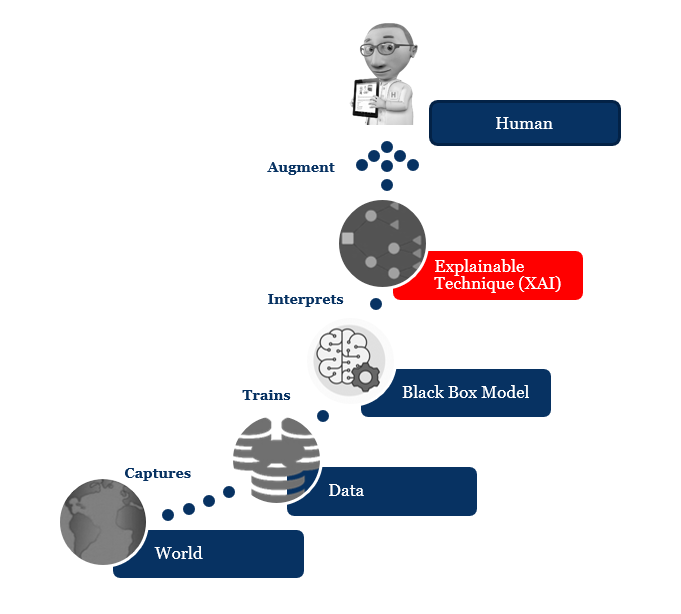
\includegraphics[scale=0.35]{src_img/explainCouche.png}
\caption{Position de la sur-couche explicative dans le processus de prédiction. \textit{Source : \cite{kdCouche}}}
\label{explainCouche}
\end{figure}
\paragraph{}Différents outils proposent une approche permettant de livrer des éléments de compréhension approximatif pour un modèle boite noire simple. Nous allons présenter les deux outils les plus populaires, LIME et SHAP.
\subsection{LIME}
\paragraph{}LIME signifie Local Interpretable Model-Agnostic Explanations (explications locales interprétables par modèle-agnostique). L'objectif est donc de fournir une interprétation local à un modèle de classification ou de régression (model agnostic) en se basant sur l’importance des variables comme vu précédemment. L'idée est de sonder la boite noire autant de fois que nécessaire en perturbant la donnée d'entrée ce qui aura pour effet de produire un résultat différent à chaque fois. Pour une prédiction d'image, nous devons récupérer l'image d'entrée pour laquelle nous voulons expliquer la prédiction et définir une multitude de zones perturbations qui seront affichées ou non comme le montre la figure \ref{perturbationExemple}.
\begin{figure}[h]
\centering
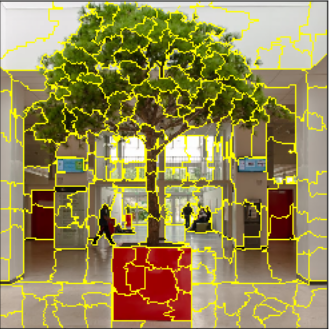
\includegraphics[scale=0.6]{src_img/perturbationExemple.png}
\caption{Exemple de zones de perturbations sur une image}
\label{perturbationExemple}
\end{figure}
\paragraph{}À partir de ces zones perturbations, nous allons générer une multitude d'image en cachant ou non chaque zone et les donner en entrée à notre modèle (entre cinquante et cent-cinquante images dans la plupart des cas). Il faudra donc stocker les prédictions effectuées par notre modèle pour chaque perturbation. Une fois que toutes les perturbations sont effectuées il est alors possible de récupérer les coefficients qui composent la droite de la régression linéaire et ainsi de déduire l'importance des zones de perturbations dans la prédiction. Notre exemple porte sur une image, mais LIME accepte aussi des données d'entrée de type tabulaire ou textuel et le principe reste le même.

\paragraph{}Par exemple dans la figure \ref{limeExemple} tirée de l'article original de la présentation de LIME\cite{limePaper} : L'image originelle (a) est donnée à notre boite noire qui prédit "Guitare électrique", "Guitare acoustique" et "Labrador". Nous constatons que le modèle s'est trompé sur la reconnaissance de la guitare électrique et nous utilisons LIME afin de comprendre ce qu'il s'est passé. LIME va prendre notre image (a) et la dériver de plusieurs façons en cachant certaines parties et envoyer ces nouvelles images à notre modèle. Le but étant de trouver les parties qui une fois cachées font que le modèle ne prédit plus la même chose. Puis une fois les trois classes trouvées, nous obtenons une explication où l'on voit les parties de l'image aillant joué un rôle dans la prédiction de chaque labels de notre modèle.
\begin{figure}[h]
\centering
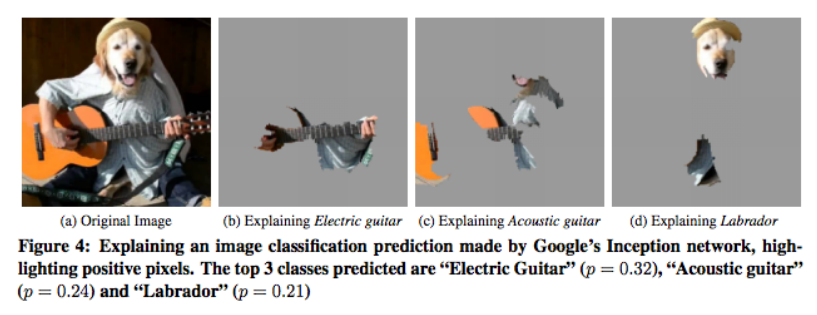
\includegraphics[scale=0.35]{src_img/limeExemple.png}
\caption{Source : LIME Paper \cite{limePaper}}
\label{limeExemple}
\end{figure}
\paragraph{}Une librairie Python est disponible afin d'utiliser l'algorithme LIME simplement sur nos modèles. Cette librairie a été créée par Marco Tulio Ribeiro qui est un des auteurs du papier original de LIME \cite{limePaper}, le code source de cette librairie est disponible sur le GitHub de son auteur \cite{limeDepot}. Cette librairie, disponible via le gestionnaire de paquets "pip", rend l'interprétation local d'un modèle très accessible, elle met à notre disposition entre autre trois méthodes majeures : LimeTabularExplainer, LimeImageExplainer et LimeTextExplainer permettant de fournir une explication local à tout type de données d'entrées. Nous aurons, dans la partie application, l'occasion d'utiliser LIME afin de voir s'il pourrait servir à rendre nos modèles de classification plus fiable.

\subsection{SHAP}
\paragraph{}Un an après la sortie de LIME, un nouvel outil fait son apparition afin de compenser entre autre le fait de ne pas pouvoir fournir une interprétation globale, cet outil s'appelle SHAP. SHAP signifie SHapley Additive exPlanations, c'est une méthode permettant de fournir une interprétation globale ou local à notre modèle. Cette méthode est basée sur la valeur de Shapley issus de la théorie des jeux, il est donc nécessaire dans un premier temps d'expliquer brièvement cette valeur de Shapley.\par
La valeur de Shapley introduit par Shapley en 1953, permet de repartir les gains équitablement dans un jeu coopératif. Le but étant que tous les joueurs coopérant ensemble reçoivent un certain gain en fonction de leur contribution.

\paragraph{}Proposée par Lundberg et al. dans l'article \cite{shapLast} faisant suite à l'article \cite{shapFirst}, SHAP reprends l'idée de la valeur de Shapley afin d'expliquer toutes sortes de modèle de machine learning. Le but étant d'associer une valeur égale à la contribution dans la prédiction de chaque caractéristique d'entrées. SHAP commence donc par déduire la contribution des caractéristiques pour chaque instance et moyenne les résultats obtenus afin de donner la contribution globale de chacune de ces caractéristiques

\paragraph{}Prenons par exemple un modèle permettant de prédire le prix d'un logement. Une multitude de caractéristiques sont données en entrés à notre modèle afin d'estimer le prix du logement, le but de SHAP est donc de définir pour chacune de ces caractéristiques leur impact monétaire sur le prix final du logement. Il interrogera donc la boite noire avec une multitude de cas différents afin d'isoler le prix de chaque caractéristique. Prenons le cas de la figure \ref{shapleyExemple} où l'on veut expliquer la prévision de 310 000 euros pour un logement de 50m2, au premier étage, près d'un parc et où les animaux sont interdits.

\begin{figure}[h]
\centering
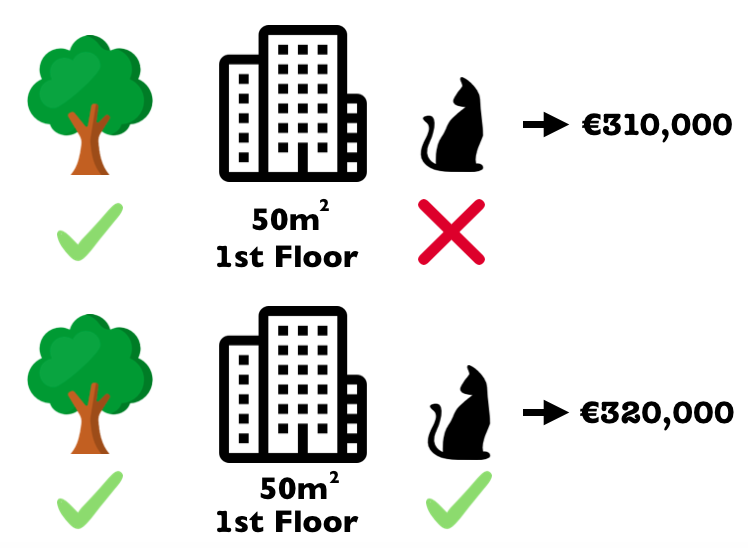
\includegraphics[scale=0.3]{src_img/shapleyExemple.png}
\caption{Exemple de l'explication du coût d'un logement avec SHAP. \textit{Source : \cite{molnar2019}}}
\label{shapleyExemple}
\end{figure}

\paragraph{}SHAP va donc recréer la même l'instance et la donner en entrée à la boite noire en autorisant les animaux afin d'en déduire le coût (dans notre exemple 10 000 euros). Cette opération sera effectuée sur toutes les caractéristiques du problème afin de trouver la contribution de chacune pour chacune des instances de notre jeu de donnée. L'interprétation globale sera ensuite donnée en faisant la moyenne de ces contributions. Cela peut sembler trivial dans cet exemple mais il peut exister des dépendances entre les caractéristiques qui modifient leurs coût en fonction de la présence ou non d'une ou plusieurs autre(s) caractéristique(s).

\paragraph{}Une librairie Python est disponible afin d'utiliser SHAP simplement sur nos modèles. Cette librairie a été créée par Scott Lundberg qui est un des auteurs des papiers originaux de SHAP cités plus haut, le code source de cette librairie est disponible sur le GitHub de son auteur \cite{shapDepot}. Cette librairie, disponible via le gestionnaire de paquets "pip", rend l'interprétation global et local et d'un modèle très accessible. Elle met à notre disposition différent types d'explicateurs permettant de fournir une explication global et local à différents types de boites noires et pour différents types de données d'entrées. Elle met aussi à notre disposition plusieurs graphiques permettant d'illustrer ses interprétations, ce qui simplifie la compréhension et la rend plus agréable.  Nous aurons, dans la partie application, l'occasion d'utiliser la librairie python de SHAP et de voir des exemples de graphiques généré dans l'objectif de savoir si SHAP peut servir à détecter des problèmes d'ordre discriminatoire.


\subsection{Limites de ces implémentations}
\paragraph{}Aujourd'hui, de nombreuses implémentations de ces méthodes sont utilisées, mais elles essuient aussi quelques critiques et ne conviennent pas dans tous les cas de figures. Premièrement, ces algorithmes représentent un coût non négligeable. Ces méthodes basées sur des simulations et interrogeant notre modèle plusieurs fois pour une seule prédiction, peuvent poser des problèmes de performances lorsque l'on manipule un très grand nombre de données. Aussi la pertinence des explications fournies sont sujettes à débat, en effet ce sont des approximations et rien ne nous garantis que ces explications correspondent réellement au fonctionnement de notre modèle. Ces explications pourraient même donner l'effet inverse à celui escompté, en effet on peut arriver dans des cas où l'on fait confiance à notre modèle grâce à ces explications alors qu'elles ne sont pas fondées et ainsi prendre une décision critique appuyée sur une explication erroné.

\paragraph{}Il est donc nécessaire d'utiliser ces algorithmes avec parcimonie et en aillant bien conscience qu'ils ne fournissent que des approximations de notre problème. Mais ce genre d'approches sont très bénéfiques pour la recherche, elles nous permettent d'apporter de nouvelles solutions ainsi que de mettre en lumière de nouvelles problématiques.
